\documentclass{beamer}

\usetheme{Boadilla}

\newcommand{\bi}{\begin{itemize}}
\newcommand{\ei}{\end{itemize}}
\newcommand{\be}{\begin{enumerate}}
\newcommand{\ee}{\end{enumerate}}
\newcommand{\bc}{\begin{center}}
\newcommand{\ec}{\end{center}}
\newcommand{\bd}{\begin{description}}
\newcommand{\ed}{\end{description}}
\newcommand{\I}{\item}
\newcommand{\f}{\frame}
\newcommand{\ft}{\frametitle}

\title{Offline Software Overview}
\subtitle{GlueX Collaboration Meeting}
\author[Mark Ito]{Mark M.\ Ito}
\date{February 19, 2016}
\institute[JLab]{Jefferson Lab}

\begin{document}

\f{\titlepage}

\f{\ft{Simulations for Spring 2016 Data}
  \bi
  \I Recent software changes incorporated
  \I Production has started
  \I Using SWIF-based system
  \ei
}

\f{\ft{Auto-Build and Test on Pull Request}
  \bi
  \I Sean introduced idea, MMI helped with JLab-side build scripts, Nathan added reconstruction
  \I new pull requests exist on a branch
  \I branches are checked out, compiled, and linked, log files searched for errors
  \I if build succeeds, a reconstruction test is run on small data file (real data), success evaluated
  \I result reported as comment to pull request page
  \ei
}

\f{\ft{Run Numbers: jump to the next round number}
  \bi
  \I Sean raised the issue, Justin gave example he had seen
  \I current run started with run 10,000; Fall run will start with run 20,000
  \I allows prediction of future run ranges; useful for simulation
  \I provides rough identification of run period via run number
  \ei
}

\f{\ft{Geant4}
  \bi
  \I David has demonstrated scaling of multi-threaded execution with out-of-the-box G4 version. (CPPsim)
  \I Work on hit generation continues (HDGeant4)
  \ei
}

\f{\ft{C++ Code Analyzer}
\bi
\I David implemented this
\I based on Clang/LLVM
\I reports questionable passages of code
\I runs nightly: {\tt https://halldweb.jlab.org/scan-build/LATEST/}
\ei
}

\f{\ft{C++ Code Analyzer}
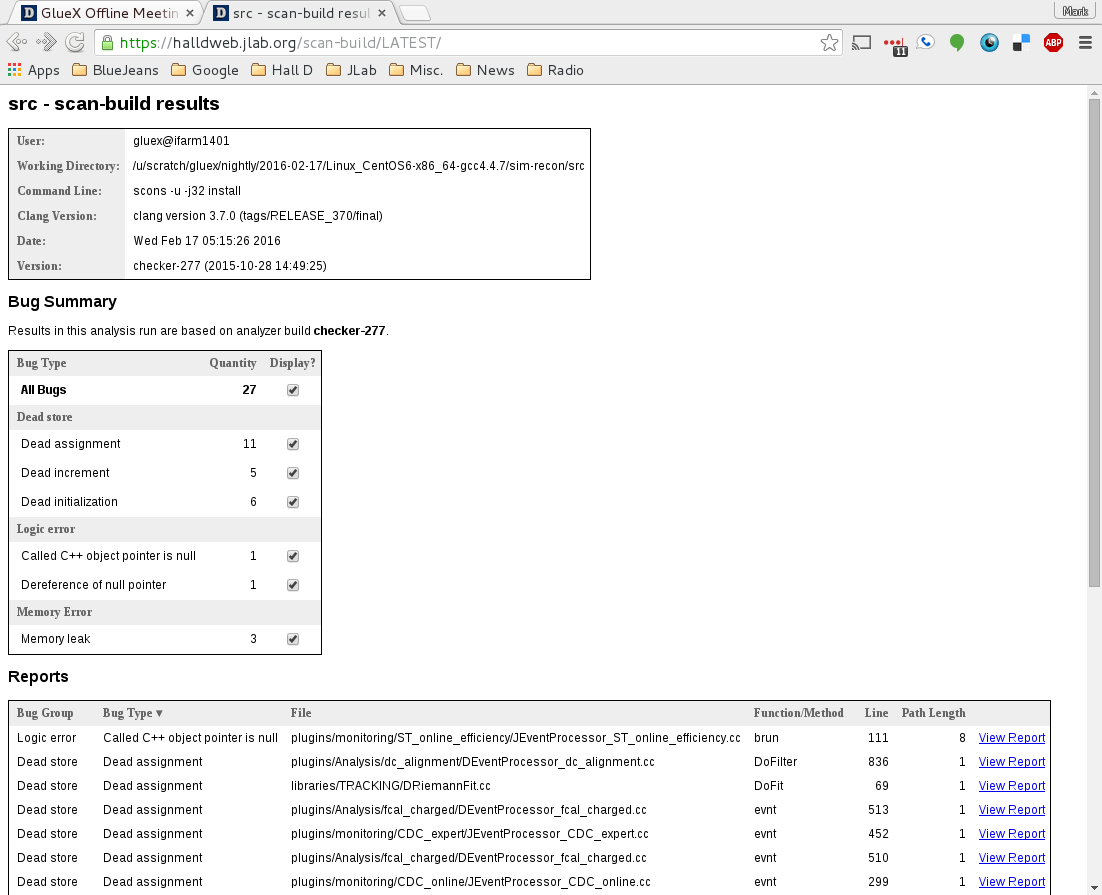
\includegraphics[width=4.5in]{code_analyzer_1.png}
}

\f{\ft{C++ Code Analyzer}
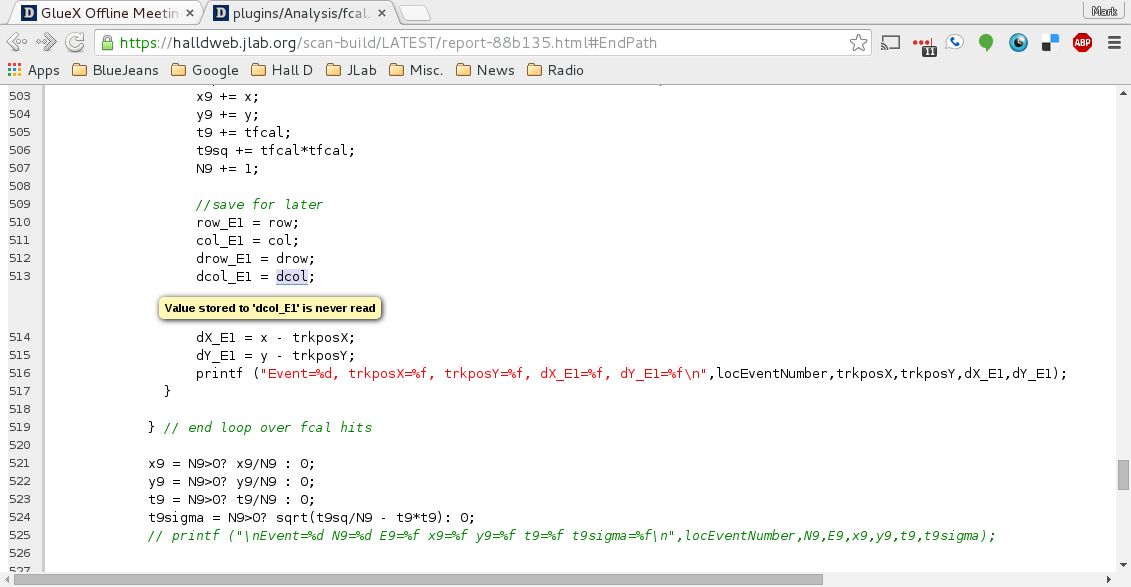
\includegraphics[width=4.5in]{code_analyzer_2.png}
}

\f{\ft{RCDB vs. CCDB for Offline Reconstruction/Analysis}
  \be
  \I Write a C++ API for the RCDB
  \I Copy data from the RCDB to the CCDB for offline use
  \ee
}

\f{\ft{Compiler Upgrade}
\bc
\begin{tabular}{ll}
\bf Site & \bf GCC version \\
\hline
JLab &			4.4.7, 4.9.2 available \\
UConn &			4.4.7 \\
Northwestern &		4.4, could go to 4.8 \\
MEPhI	&		4.9 \\
CMU	&		4.4.7, could go to 4.9.2 \\
Athens	&		4.8.4 \\
Regina	&		4.4.7 \\
Open Science Grid &	4.4.7, option for 4.9.2
\end{tabular}
\ec
\bi
\I New C++11 language features available in 4.8 and higher
\I Some developers would like to use modern features
\I Each computer used to compile code would have to upgrade
\I Proposal: go to 4.9.2
\I When?
\ei
}

\f{\ft{New releases}
  \bi
  \I sim-recon 1.6.0, 1.7.0, 1.8.0, 1.9.0
  \I HDDS 3.4, 3.5
  \I JANA 0.7.4p2
  \I CCDB 1.06.01
  \I Xerces-C++ 3.1.2
  \ei
}

\f{\ft{Odds and Ends}
  \bi
  \I JANA status bits: identify event source
  \I DL1Trigger bits: identify which trigger(s) fired
  \I No more farm62 nodes (CentOS 6.2), using 6.5 exclusively
  \I New Lustre-based work disk: {\tt /work/halld}
  \I New Traditional work disk: {\tt /work/halld2}
  \I Volatile space: 10 TB to 20 TB
  \I New Private Wiki: {\tt https://halldweb.jlab.org/wiki-private/}
  \I Git usage regularized
  \ei
}

\f{\ft{New hypernews forum coming}
  \bi
  \I Discussions of low-level software/computing issues
  \I Access via webpage and/or email
  \I Questions can be answered in a public forum
  \I Forum naming contest underway:
    \bi
    \pause
    \I ``GlueX Software Help Forum''
    \pause
    \I ``Dumb Offline Software Questions''
    \pause
    \I ``The Clueless on the Farm Forum''
    \pause
    \I ``Seg-Fault of the Day''
    \pause
    \I ``The `Doctor Mattione Will See You Now' Forum''
    \pause
    \I ``Free Video Streaming Recommendations''
    \ei
  \ei
}

\end{document}
